\chapter{Návrh implementace}
\label{ChapterImplementace}

Samotná implementace je rozdělena do dvou částí:
\begin{enumerate}
	\item Komunikace RaspberryPi přes rozšiřující desku UniPi s bezdrátovým modulem a pomocí něj s poskytnutými WM-Bus zařízeními.
	\item Zachytávání šifrované i nešifrované komunikace s WM-Bus zařízeními. 
	\item Analýza, dešifrování, parsování a uložení zachycených dat. 
	\item Vizualizace získaných dat.
\end{enumerate}

Jelikož žádný z dostupných softwarů pro UniPi nepodporuje daný bezdrátový modul, ani UART zařízení obecně, je nutné tuto komunikaci implementovat již na~úrovni operačního systému.

%%%%%%%%%%%%%%%%%%%%%%%%%%%%%%%%%%%%%%%%%%%%%%%%%%%%%%%%%%%
%%%%%%%%%%%%%%%%%%%%%%%%%%%%%%%%%%%%%%%%%%%%%%%%%%%%%%%%%%%
%%%%%%%%%%%%%%%%%%%%%%%%%%%%%%%%%%%%%%%%%%%%%%%%%%%%%%%%%%%
%%%%%%%%%%%%%%%%%%%%%%%%%%%%%%%%%%%%%%%%%%%%%%%%%%%%%%%%%%%

\section{Výběr OS}
Jako operační sytém je využita aktuální verze Raspbianu Jessie s datem vydání 2017-03-02. UART rozhraní se na RaspberryPi verze 1 a 2 nachází v \texttt{/dev/ttyAMA0}. To~se~ale~v~případě RaspberryPi 3 odkazuje na integrovaný BT modul a původní sériový port je zde v \texttt{/dev/ttyS0}. Samotné UART rozhraní je ale ve výchozím nastavení Raspbianu zakázáno.

Pro zpřístupnění UART rozhraní je nutné provést úpravy jeho konfigurace:


\begin{enumerate}
	\item Nejdříve je nutné provést kompletní aktualizaci Raspbianu, tedy v konzoli spustit posloupnost příkazů:
	
	\begin{lstlisting}[style=MyCodeBash]
		sudo apt update
		sudo apt upgrade
		sudo apt dist-upgrade
	\end{lstlisting}
					
	\item Poté je potřeba v \texttt{/boot/config.txt} změnit položku \texttt{ENABLE\_UART} na hodnotu 1. Tím dojde k zpřístupnení sběrnice UART. Tato položka může být v budoucnu při aktualizaci Raspbianu přepsána, proto při prvním náznaku nefunkčnosti, je potřeba tuto položku zkontrolovat jako první.
	\item V souboru \texttt{/boot/cmdline.txt} je potřeba odebrat text \texttt{console=ttyAMA0, 115200}, aby při startování systému nedocházelo k výpisu do sériové linky. 
	\item V případě, že se jedná o RaspberryPi verze 3, je potřeba do \texttt{/boot/config.txt} dopsat položku \texttt{dtoverlay=pi3-miniuart-bt}, která zakáže BT na mini-UART a provede přemapování zpět na \texttt{/dev/ttyAMA0}. Tento krok je takto řešený z důvodu kompatibility, kdy je sériová komunikace směrována přes \texttt{/dev/ttyAMAO} nezávisle na použité verzi RaspberryPi.
\end{enumerate}

Po každém z těchto kroků je doporučován restart zařízení. Kroky byly otestovány pouze na výše zmíněné verzi Raspbianu a v jiných distribucích se monou mírně lišit. Úspěšnost provedení těchto kroků lze zkontrolovat pomocí zadání příkazu konzole \texttt{sudo dmesg | grep tty} jehož výstup by měl být následující:
					
	\begin{lstlisting}[style=MyCodeBash]
		[0.000974] console [tty1] enabled
		[0.130442] 20201000.uart: ttyAMA0 at MMIO 0x20201000 
		(irq = 81, base_baud = 0) is a PL011 rev2
	\end{lstlisting}
	\vspace{-20pt}


%%%%%%%%%%%%%%%%%%%%%%%%%%%%%%%%%%%%%%%%%%%%%%%%%%%%%%%%%%%
%%%%%%%%%%%%%%%%%%%%%%%%%%%%%%%%%%%%%%%%%%%%%%%%%%%%%%%%%%%
%%%%%%%%%%%%%%%%%%%%%%%%%%%%%%%%%%%%%%%%%%%%%%%%%%%%%%%%%%%
%%%%%%%%%%%%%%%%%%%%%%%%%%%%%%%%%%%%%%%%%%%%%%%%%%%%%%%%%%%

\section{Výběr programovacího jazyka}
Jelikož primárním jazykem využívaným na platformě RaspberryPi je Python, který již obsahuje knihovny pro sériovou komunikaci, je současný kód napsán v programovacím jazyce Python 3.

%%%%%%%%%%%%%%%%%%%%%%%%%%%%%%%%%%%%%%%%%%%%%%%%%%%%%%%%%%%
%%%%%%%%%%%%%%%%%%%%%%%%%%%%%%%%%%%%%%%%%%%%%%%%%%%%%%%%%%%
%%%%%%%%%%%%%%%%%%%%%%%%%%%%%%%%%%%%%%%%%%%%%%%%%%%%%%%%%%%
%%%%%%%%%%%%%%%%%%%%%%%%%%%%%%%%%%%%%%%%%%%%%%%%%%%%%%%%%%%

\section{Nastavení komunikačního modulu a čidla}

Před samotným vyčítáním dat bylo potřeba zjistit či nastavit přenosové parametry všech použitých zařízení:

\begin{itemize}
	\item Komunikační modul IQRF nastaven do módu T1 ve funkci skeneru.
	\item Čidlo Weptech je nastaveno do módu T1 s intervalem zasílání 1 minuta. 
	\item Modul Bonega je nastaven do módu T1 se zapnutým šifrováním AES128 v~módu 5 a s intervalem zasílání 20-24 sekund v odpočtovém období a intervalem 4 minuty mimo odpočtové období.
	\item Elektroměr ZPA je nastaven do módu T2 s intervalem vysílání 1 minuta.
	\item Měřič Kamstrup je nastaven do módu T1 s intervalem vysílání 15 minut.
\end{itemize}

%%%%%%%%%%%%%%%%%%%%%%%%%%%%%%%%%%%%%%%%%%%%%%%%%%%%%%%%%%%
%%%%%%%%%%%%%%%%%%%%%%%%%%%%%%%%%%%%%%%%%%%%%%%%%%%%%%%%%%%
%%%%%%%%%%%%%%%%%%%%%%%%%%%%%%%%%%%%%%%%%%%%%%%%%%%%%%%%%%%
%%%%%%%%%%%%%%%%%%%%%%%%%%%%%%%%%%%%%%%%%%%%%%%%%%%%%%%%%%%

\section{Zajištění dedikovaného běhu}
Pro zajištění běhu aplikace nezávisle na typu provozu RaspberryPi bude daný program spouštěn ihned po startu operačního systému pomocí příkazu screen. Je tedy nutné ho doinstalovat:
 
\begin{lstlisting}[style=MyCodeBash]
		sudo apt install screen		
	\end{lstlisting}


%%%%%%%%%%%%%%%%%%%%%%%%%%%%%%%%%%%%%%%%%%%%%%%%%%%%%%%%%%%
%%%%%%%%%%%%%%%%%%%%%%%%%%%%%%%%%%%%%%%%%%%%%%%%%%%%%%%%%%%
%%%%%%%%%%%%%%%%%%%%%%%%%%%%%%%%%%%%%%%%%%%%%%%%%%%%%%%%%%%
%%%%%%%%%%%%%%%%%%%%%%%%%%%%%%%%%%%%%%%%%%%%%%%%%%%%%%%%%%%

\section{Zajištění podpory šifrování}
Některá ze zařízení používají pro přenos dat šifrování. Pro zajištění podpory šifrování byla zvolena knihovna PyCrypto, která podporuje jak šifrování DES tak i AES. 
Umožňuuje pohodlnou implementaci AES128 pomocí jazyku Python3. Na rozdíl od ostatních knihoven není závislá na balíčku OpenSSL a je součástí repozitářů Raspbianu. 

Je nutné doinstalovat nezbytné balíčky:	
 
\begin{lstlisting}[style=MyCodeBash]
		sudo apt install python-crypto
		sudo apt install python-dev
	\end{lstlisting}
	\vspace{-20pt}

%%%%%%%%%%%%%%%%%%%%%%%%%%%%%%%%%%%%%%%%%%%%%%%%%%%%%%%%%%%
%%%%%%%%%%%%%%%%%%%%%%%%%%%%%%%%%%%%%%%%%%%%%%%%%%%%%%%%%%%
%%%%%%%%%%%%%%%%%%%%%%%%%%%%%%%%%%%%%%%%%%%%%%%%%%%%%%%%%%%
%%%%%%%%%%%%%%%%%%%%%%%%%%%%%%%%%%%%%%%%%%%%%%%%%%%%%%%%%%%

\section{Zpracování dat}

\subsection{Nešifrovaný přenos}

Jednoduchým spuštěním komunikačního modulu v módu skeneru byl zachycen telegram

\begin{lstlisting}[style=MyCodePHP]
			32002E44B05C10000000021B7A620800002F2F0A6699010AFB1
			A930202FD971D01002F2F2F2F2F2F2F2F2F2F2F2F2F459e0D0A
\end{lstlisting}

který byl pomocí datasheetu použitého komunikačního modulu~\cite{ModulIQRF} a~čidla~\cite{CidloWeptech} analyzován, a přehledně zobrazen do Tab. \ref{PacketTableAnalysis}, vycházející z~Tab.~\ref{TabulkaTelegramWeptech}.

\subsection{Šifrovaný přenos}

V okamžiku, kdy bylo zařízení přepnuto do šifrovaného módu dle Tab.~\ref{TablukaSETUP}, byl zachycen šifrovaný telegram

\begin{lstlisting}[style=MyCodePHP]
			32002E44B05C10000000021B7AC40820053ED44A38A9C3C86F5
			8210F9B979353C39DC1D5E0C873EB81994D28C099EF1D55B008
\end{lstlisting}

který byl pomocí datasheetů použitého komunikačního modulu \cite{ModulIQRF} a normy~\cite{Norma1,NormaFIPS} analyzován a byly vyparsovány položky nezbytné pro dešifrování dat:
\begin{itemize}
	\item 30-33 pro informaci použitém šifrování,
	\item 8-25 pro sestavení inicializačního vektoru a
	\item 38-93 pro šifrovanou část dat.
\end{itemize}

\newpage

Poté byla daná data v souladu s normou \cite{NormaFIPS} dešifrována dle Kap.~\ref{KapitolaDesifrovani} a byl získán dešifrovaný telegram:



\begin{lstlisting}[style=MyCodePHP]
			32002E44B05C10000000021B7AC40800002F2F0A6699010AFB1
			A930202FD971D01002F2F2F2F2F2F2F2F2F2F2F2F2F879e0D0A
\end{lstlisting}

který je až na číslo přístupu a CRC shodný s předchozím nešifrovaným telegramem. Nyní tedy lze dešifrovaná data vyparsovat jako při nešifrovaném přenosu popsaném v předchozí kapitole.

\begin{table}[!ht]
\centering
\vspace{-10pt}
\caption{Rozklíčovaný zachycený paket}
\resizebox{\textwidth}{!}{%
\label{PacketTableAnalysis}
\begin{tabular}{|c|c|c|l|l|c|l|}
\hline
\textbf{Pozice} & \textbf{Bajty} & \multicolumn{1}{c|}{\textbf{Pole}} & \multicolumn{1}{c|}{\textbf{Popis}} & \textbf{Hodnota} & \textbf{Vyjádření} & \multicolumn{1}{c|}{\textbf{Význam pro uživatele}} \\ \hline \hline
4 & 2E & L-Field & Délka telegramu & 2Eh & 46 & Paket má 46 bytů \\ \hline
6 & 44 & C-Field & Typ telegramu & 44h & 44 & Paket je typu SND-NR \\ \hline
8 & B0 & \multirow{2}{*}{M-Field} & \multirow{2}{*}{Výrobce zařízení} & B0h & \multirow{2}{*}{5CB0}& \multirow{2}{*}{Výrobcem je Weptech}  \\ \cline{1-2} \cline{5-5} 
10 & 5C &  &  & 5Ch &  &  \\ \cline{1-3} \cline{4-7}
12 & 10 &  \multirow{6}{*}{A-Field} & \multirow{4}{*}{Sériové číslo} & 10h & \multirow{4}{*}{10} & \multirow{4}{*}{Výrobní číslo je 00000010 } \\ \cline{1-2}  \cline{5-5} 
14 & 00 &  &  & 00h &  &  \\ \cline{1-2}  \cline{5-5}  
16 & 00 &  &  & 00h &  &  \\ \cline{1-2}  \cline{5-5} 
18 & 00 & &  & 00h &  &  \\ \cline{1-2}  \cline{4-7} 
20 & 02 & & Verze zařízení & 01h & 2 & Druhá verze \\ \cline{1-2}  \cline{4-7} 
22 & 1B & & Typ zařízení & 1Bh & 1B & Pokojové čidlo \\ \hline
24 & 7A & CI-Pole & Odpověd zařízení & 7Ah & 7A & M-Bus protokol \\ \hline
26 & 62 & Access Number & Číslo přístupu & 41h & 214 & 214. přístup \\ \hline
28 & 08 & Status & Status zařízení & 08h & 8 & Trvalá chyba - sabotáž\\ \hline
30 & 00 & \multirow{2}{*}{\begin{tabular}[c]{@{}c@{}}Configuration\\ Word \end{tabular}} & \multirow{2}{*}{Šifrování AES} & \multirow{2}{*}{00h} & \multirow{2}{*}{00} & \multirow{2}{*}{Bez šifrování} \\ \cline{1-2}
32 & 00 &  &  &  &  &  \\ \hline
34 & 2F & \multirow{2}{*}{\begin{tabular}[c]{@{}c@{}}AES\\ Verification \end{tabular}} & \multirow{2}{*}{Ověření AES} & \multirow{2}{*}{2Fh} & \multirow{2}{*}{2F} &  \multirow{2}{*}{Kontrola v pořádku} \\ \cline{1-2}
36 & 2F &  & &  &  &  \\ \hline
38 & 0A & \multirow{4}{*}{1. data block} & DIF: datový typ & 0Ah & 0A & 2 cifry BCD = 16-bit integer \\ \cline{1-2} \cline{4-7}
40 & 66 &  & VIF: měřená veličina & 66h & 66 & Teplota v \degree\,C\textsuperscript{-1} \\ \cline{1-2} \cline{4-7}
42 & 99 &  & \multirow{2}{*}{DATA: hodnota} & 99h & \multirow{2}{*}{0199} & \multirow{2}{*}{Teplota je 19.9\degree\,C} \\ \cline{1-2} \cline{5-5}
44 & 01 &  &  & 01h &  &  \\ \hline
48 & 0A & \multirow{4}{*}{2. data block} & DIF: datový typ & 0Ah & 0A & 2 cifry BCD = 16-bit integer \\ \cline{1-2} \cline{4-7}
50 & 1A &  & VIF: měřená veličina & 1Ah & 1A & Relativní vlhkost v \%\textsuperscript{-1} \\ \cline{1-2} \cline{4-7}
52 & 93 &  & \multirow{2}{*}{DATA: hodnota} & 93h & \multirow{2}{*}{0293} & \multirow{2}{*}{Vlhkost je 29.3\,\%} \\ \cline{1-2} \cline{5-5} 
54 & 02 &  &  & 02h &  &  \\ \hline
58 & FD & \multirow{5}{*}{3. data block} & DIF: datový typ & FDh & FD & 2 cifry BCD = 16-bit int/bool \\ \cline{1-2} \cline{4-7}
60 & 02 &  & DIFE: rozš. tabulka & 02h & 02 &  Bude následovat VIFE kód \\ \cline{1-2} \cline{4-7}
62 & 1D &  & VIF: Norma & 1Dh & 1D & Norma dle výrobce \\ \cline{1-2} \cline{4-7}
64 & 01 &  & VIFE: Příznak sabotáže & 00h & 1 & Čidlo bylo otevřeno \\ \cline{1-2} \cline{4-7}
66 & 00 &  & VIFE: Příznak baterie & 00h & 0 & Baterie je nabitá \\ \hline
94 & 87 & CRC & Kontrolní součet & 87h & 135 & Hodnota kontrolního součtu \\ \hline
96 & 9e & RSSI & Síla přij. signálu& 9Eh & 158 & Síla signálu  je -51\,dBm \\ \hline \hline
\end{tabular}}
\end{table}


Z tabulky je patrné, že je nutné vyparsovat položky na následujících pozicích:
\begin{itemize}
	\item 8-23 pro informace o daném čidlu,
	\item 24-25 pro určení pořadí telegramu,
	\item 42-45 pro hodnotu naměřené teploty,
	\item 52-55 pro hodnotu naměřené vlhkosti,
	\item 64-67 pro kontrolu stavu čidla a
	\item 96 pro úroveň signálu.	
\end{itemize}

Jejich následnou správnou interpretací dle specifikace (zohlednění uložení LSB, převod hexadecimálních hodnot na dekadické, \ldots) předat k dalšímu zpracování či~uložení do databáze.


\section{Zajištění uložení dat}
\label{SectionUlozeniDatabaze}
Zachycená a naměřená data se ukládají do databáze k pozdějšímu zpracování či~vizualizaci. Zvolena byla databáze SqLite3 pro svoji jednoduchost, nenáročnost na~sytémové prostředky a možností instalace z repozitáře Raspbianu:
 
\begin{lstlisting}[style=MyCodeBash]
		sudo apt-get update
		sudo apt-get install sqlite3
	\end{lstlisting}

Byla zvolena jedna databáze se třemi tabulkami:
\begin{itemize}
	\item DEVICES - evidence známých zařízení a jejich AES klíčů.
	\item VALUES - uložení naměřených hodnot.
	\item TELEGRAMS - uložení zachycených dat a AES klíče modulu.
\end{itemize}

Strukturu tabulek, definici sloupců a vazby mezi nimi popisuje schéma na Obr.~\ref{databazovy_model}.

\begin{figure}[!ht]
  \begin{center}
    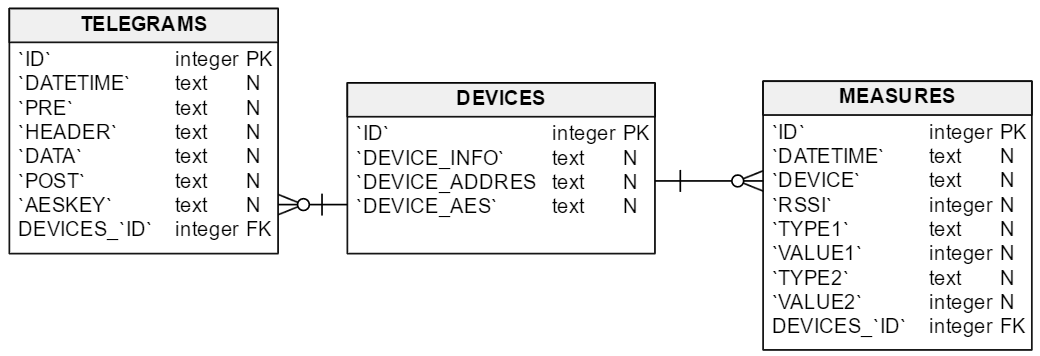
\includegraphics[scale=0.80]{obrazky/aplikace_databaze}
  \end{center}
	\vspace{-15pt}
  \caption{Model zvolené SqLite 3 databáze}
	\label{databazovy_model}
\end{figure}

Prohlížení obsahu databáze je součástí vizualizační aplikace pod záložkou \texttt{Database explorer}.

\newpage

\section{Zajištění vizualizace dat}	
\label{SectionVizualizaceDat}
Zachycená a uložená data lze vykreslovat do grafů. Zvoleno bylo Google Charts API~\cite{uvod_google_charts_api} běžící na webovém serveru Apache 2 a generovaném pomocí PHP 7. Pro tyto potřeby je nutné doinstalovat následující balíčky:
 
\begin{lstlisting}[style=MyCodeBash]
		sudo apt-get update
		sudo apt-get install apache2
		sudo apt-get install php7.0 
	\end{lstlisting}

Dále je nezbytné do umístění \texttt{$\backslash$var$\backslash$www$\backslash$html$\backslash$} nahrát zdrojové soubory visualizační aplikace. 

Prohlížení vizualizovaných dat se ve visualizační aplikaci nachází pod záložkou \texttt{Graphs Explorer}.

\section{Struktura aplikace}
Vzhledem k výše uvedeným požadavakům a technologiím byla zvolena struktura aplikace znázorněná na Obr.~\ref{AplikaceDiagram}. Diagram je pro přehlednost odlišen barevnými bloky:
\begin{itemize}
	\item modrou barvou je znázorněna kostra programu,
	\item zelenou barvou je nekonečná smyčka naslouchání dat,
	\item růžovou barvou je případné dešifrování přenášených dat,
	\item červenou barvou jsou chyby znemožnující běh programu,
	\item oranžovou barvou jsou chyby znemožňující platnou analýzu či dešifrování daného telegramu a
	\item černou barvu je řízení samotného programu.
\end{itemize}

\begin{figure}[!ht]
  \begin{center}
    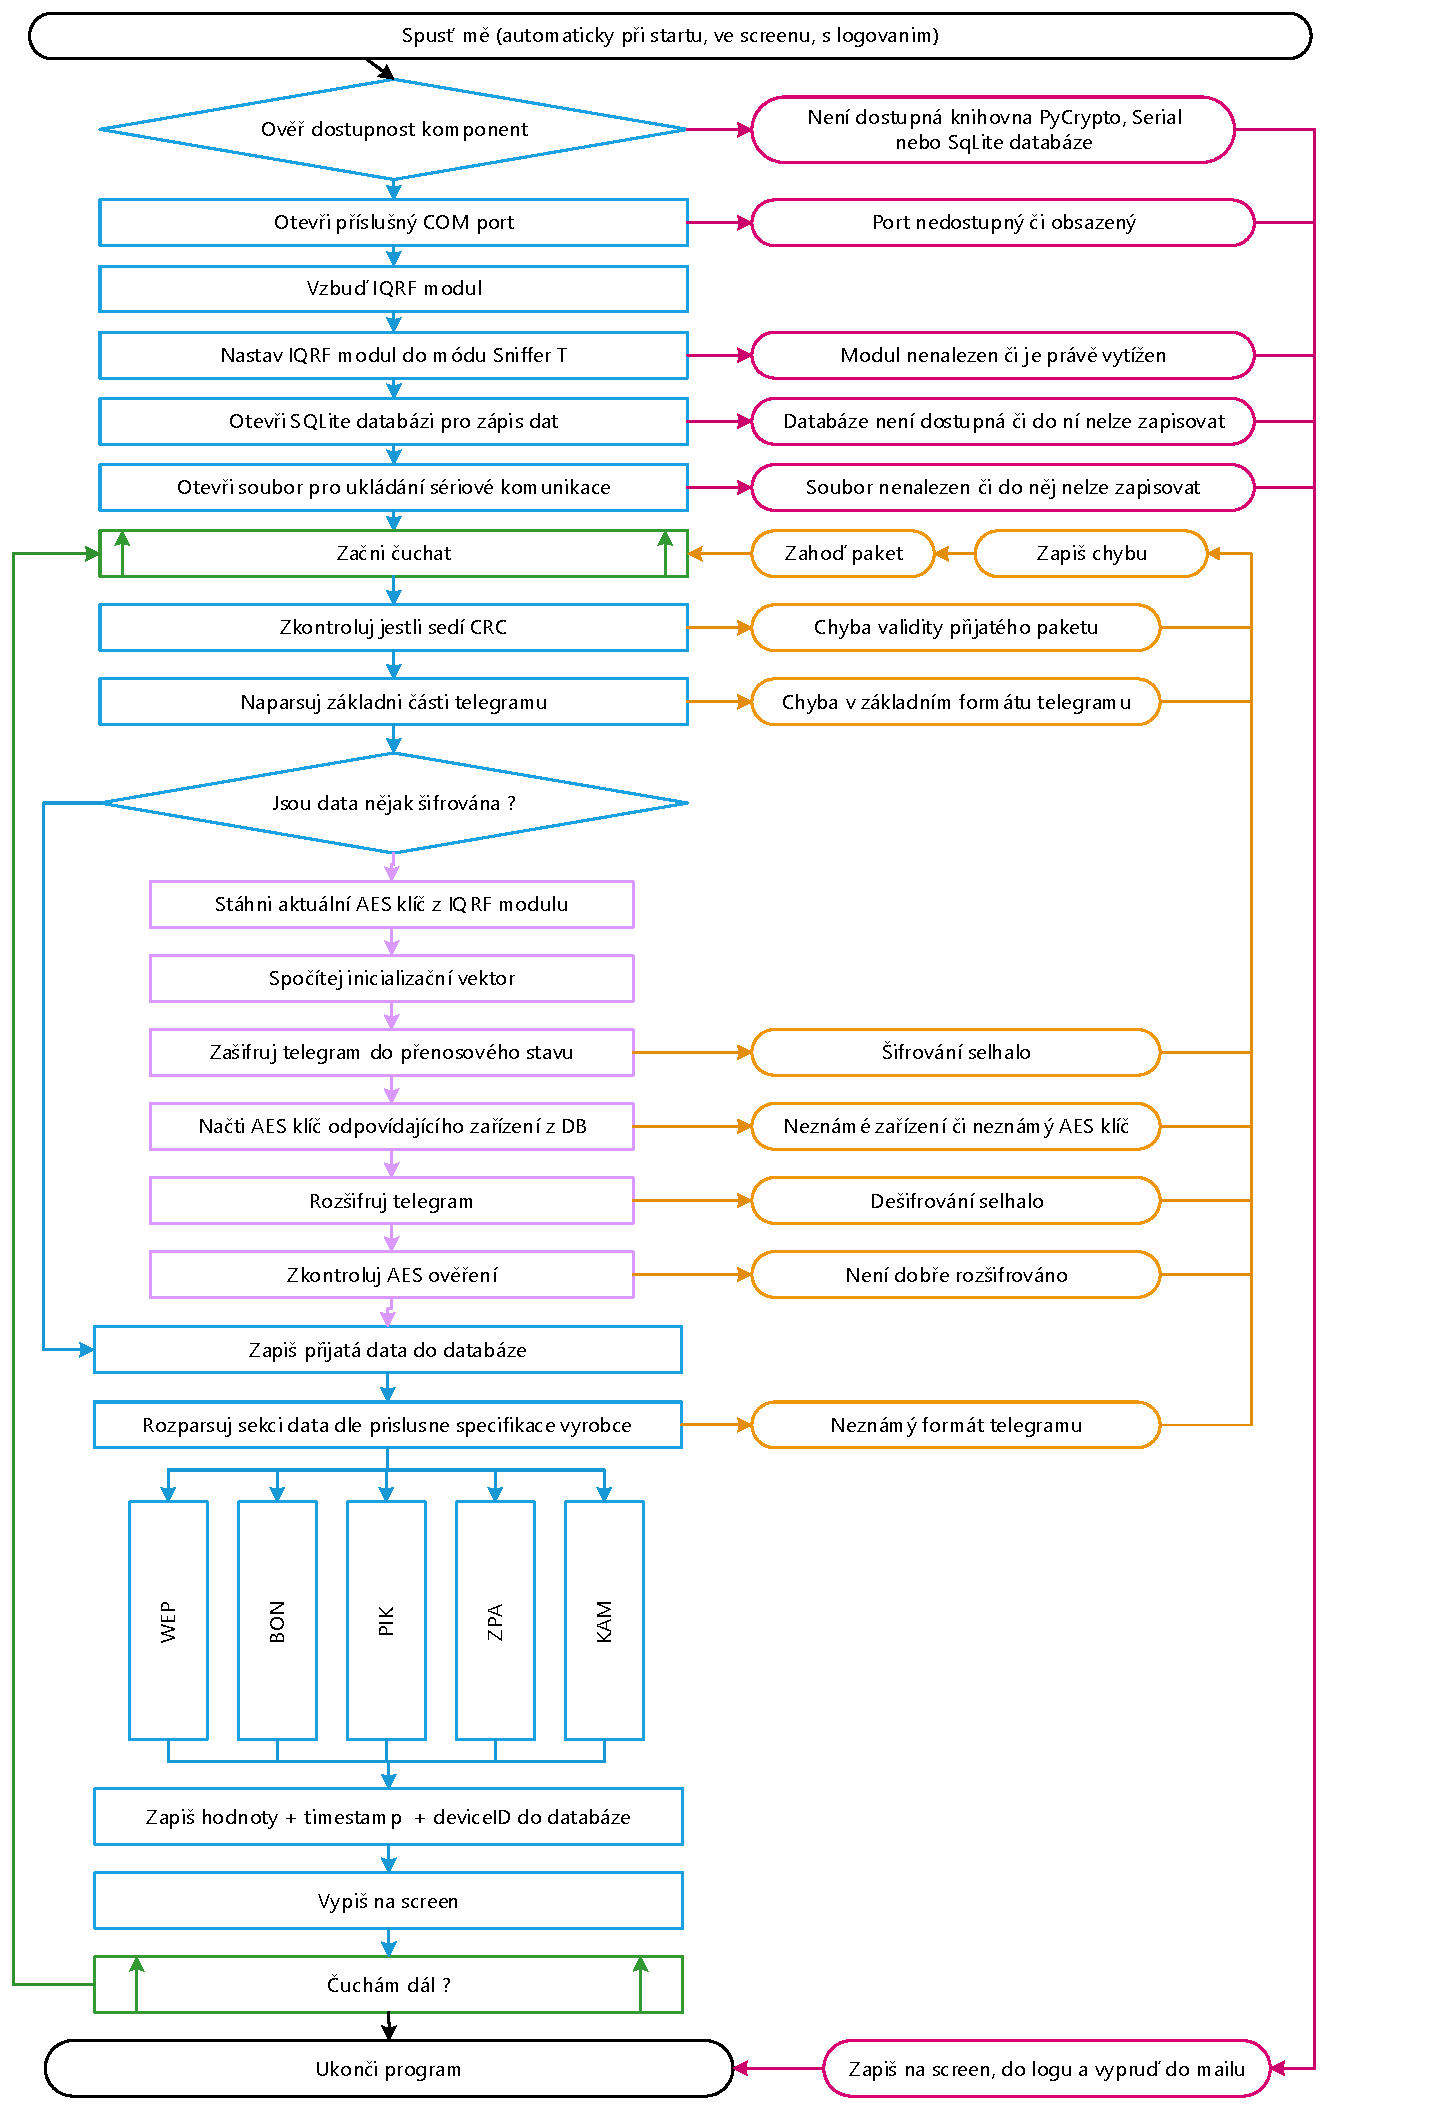
\includegraphics[scale=0.55]{obrazky/aplikace_diagram}
  \end{center}
	%\vspace{-20pt}
  \caption{Vývojový diagram aplikace pro vyčítání dat}
	\label{AplikaceDiagram}
	%\vspace{-30pt}
\end{figure}

V následujících podkapitolách budou jednotlivé bloky aplikace představeny podrobněji.

\subsection{Start programu v rámci operačního systému}
Program je nyní spouštěn automaticky po startu operačního systému interpretem jazyka Python v příkazu screen. Tímto dojde k oddělení běhu programu od ostatních aplikací, možností vzdáleného připojení ke konzolovým výstupům aplikace a nezávislosti na případných restartech zařízení. Ukončení programu nastává pouze násilným ukončením aplikace, restartem zařízení nebo závažnou chybou při startu programu. 

\subsection{Start programu z pohledu aplikace}
Program při startu kontroluje, jestli  má k dispozici všechny potřebné komponenty pro svůj běh. Program je závislý na knihovně PyCrypto, Serial nebo SQLite databázi.
Dále program kontroluje přítomnost a možnost otevření sériového portu. V~případě úspěšného otevření portu je na něj zaslán příznak pro probuzení komunikačního modulu z úsporného režimu. Po probuzení následuje příkaz, který nastaví modul do režimu skeneru v komunikačním módu T1. Pokud některá z operací selže, je zaznamenán chybový stav a dojde k ukončení programu.

\subsection{Základní kontrola a cyklus příjmu dat}
Následně dojde ke spuštění smyčky naslouchání příchozích telegramů. Každý příchozí telegram je podroben sérii kontrol, pro ověření správnosti příjmu. Jako první je telegram podroben kontrole délky odpovídající sudým násobkům. Následně je telegram podroben základní analýze položek aplikační a linkové vrstvy. Dochází ke~kontrole délky telegramu a jeho CRC součtu. Je provedena kontrola obsahu \texttt{CI}-pole, \texttt{Status} pole a \texttt{ConfigurationWord} pole. Pokud některá z položek neodpovídá, telegram je~zaevidován a aplikace se vrátí do stavu čekání na příchod dalšího telegramu.
Na~základě obsahu položky \texttt{ConfigurationWord} (viz Kap.~\ref{KapitolaConfigurationWord}) se program nadále větví na zpracování šifrovaného (Kap. \ref{KapitolaDesifrovani}) a nešifrovaného (Kap. \ref{KapitolaParsovani}) telegramu.

\subsection{Dešifrování dat}
\label{KapitolaDesifrovani}
%%%%%%%%%%%%%%%%%%%%%%%%%%%%%%%%%%%%%%%%%%%%%%%%%%%%%%%%%%
Pokud je analýzou položky \texttt{ConfigurationWord} zjištěno šifrování dat přenášených dat algoritmem AES128 CBC, je zahájen proces dešifrování dat.

Díky vnitřní implementaci IQRF modulu (zmíněno v Kap.~\ref{KapKomMody}) jsou všechny zachycené šifrované pakety automaticky rozšifrovány pomocí AES klíče nahraného v paměti modulu. Jedná se však o klíč daného modulu, nikoliv vyčítaného zařízení. Tato dešifrovaná data jsou tedy nevalidní. Celý postup dešifrování (viz Kód~\ref{CodeAES}) se tak komplikuje:

\begin{enumerate}
	\item Dojde ke stažení aktuálního AES klíče (viz Kap.~\ref{KapitolaStazeniKlice}) nastaveného v IQRF modulu, s pomocí něj a sestaveného inicializačního vektoru (viz Kap.~\ref{KapitolaInicializacniVektor})
jsou přijatá data zašifrována zpět do šifrovaného stavu jaký mají při přenosu, tedy data vyslaná daným měřícím zařízením, zašifrovaná AES klíčem daného měřícího zařízení.
	\item Pokud existuje, tak je z databáze načten odpovídající klíč příslušného měřícího zařízení a s pomocí již sestaveného inicializačního vektoru jsou data rozšifrována.
	\item Správnost rozšifrování se ověřuje pomocí kontrolních bajtů, v případě AES šifrování mají první dva bajty rozšifrovaných dat hodnotu 2Fh.
\end{enumerate}

\begin{lstlisting}[caption={Implementace AES dešifrování},captionpos=b,label=CodeAES,style=MyCodePython]
from Crypto.Cipher import AES

# Encrypt telegram with AES key from IQRF module
encryptor_back = AES.new(AES_KEY_IQRF, AES.MODE_CBC, IV=AES_IV)
TELEGRAM_CRYPTED = encryptor_back.encrypt(TELEGRAM_DECRYPTED)

# Decrypt telegram with  AES key of used device
encryptor_new = AES.new(AES_KEY_DEVICE, AES.MODE_CBC, IV=AES_IV)
TELEGRAM_ORIGINAL = encryptor_new.decrypt(TELEGRAM_CRYPTED)
\end{lstlisting}


Poté program s telegramem zachází jako s nešifrovaným, popsaným v Kap.~\ref{KapitolaParsovani}. Pokud není nalezen AES klíč odpovídajícího zařízení, pole \texttt{ConfigurationWord} obsahuje neimplementovaný algoritmus dešifrování či se proces dešifrování nezdaří, program vyvolá vyjímku, telegram je zaevidován a pokračuje se zpracováváním dalšího telegramu.

\subsection{Parsování dat}
\label{KapitolaParsovani}
Každý telegram je před svým zpracováním uložen do databáze, aby v případě potřeby (špatné dešifrování, neadekvátní dešifrovací klíč, chyba aplikace, neznámý senzor, \ldots) mohlo být provedeno opětovné zpracování daného telegramu. Poté je analyzováno M-Pole a v případě že se jedná o výrobce, jehož parsovací schéma je~v~této aplikaci implementováno, dochází k vyparsování  přenášených hodnot (viz Kód~\ref{CodeParse}). Následně v~souladu s parsovacím schématem dochází k formátování a odpovídající interpretaci získaných dat (viz Kap.~\ref{PacketTableAnalysis}). Poté jsou získaná data uložena do databáze a zobrazena uživateli na výstup konzole.


\begin{lstlisting}[caption={Ukázka parsování dat},captionpos=b,label=CodeParse,style=MyCodePython]
# Parse values from Weptech
if (sensor_manu == "WEP"):
	if parsedstring[66:68] == "01": errors = "Battery dead"
		temperature = str(int(LSB(parsedstring[42:46])) / 10)
		humidity = str(int(LSB(parsedstring[52:56])) / 10)
		# Parse values from Bonega       
elif (sensor_manu == "BON"):
	Spotreba = str(int(LSB(parsedstring[42:46]), 16))
	Cascteni = get_date(LSB(parsedstring[58:62])) + " " + get_time(LSB(parsedstring[54:58]))
\end{lstlisting}
Pokud parsování dat selže, dojde k výjimce, daný telegram je zaevidován, v jeho zpracování se již nepokračuje a aplikace se vrátí do~stavu čekání na příchod dalšího telegramu.

\subsection{Uložení dat}
\label{SectionUlozeniDatabaze2}
Správně interpretované hodnoty doplněné o časovou značku a informaci o měřícím zařízení jsou zapsány do databáze. Do této databáze se ukládají všechny příchozí validně zpracované telegramy, určené k pozdějšímu zpracování. Po doplnění o časovou značku a údaje o zařízení je možné tyto data efektivně třídit či v nich vyhledávat. Ukázka implementace je v Kódu~\ref{CodeStore}.

\vspace{10pt}

\begin{lstlisting}[caption={Ukázka ukládání dat},captionpos=b,label=CodeStore,style=MyCodePython]
db = sqlite3.connect('\MainDatabase.db')
def sql(query):
    db.execute(query)
    db.commit()
    output('SQL', query)
    return
...
sql("INSERT INTO TELEGRAMS VALUES ('"+time.strftime("%Y-%m-%d %H:%M")+"', '"+parsedstring[0:4]+"', '"+parsedstring[4:34]+"', '"+parsedstring[34:-4]+"', '"+parsedstring[-4:]+"','"+AES_IQRF_DEFAULT+"')")		
\end{lstlisting}

Prohlížení obsahu databáze je součástí vizualizační aplikace pod záložkou \texttt{Database explorer}.


\subsection{Ošetření výjimek}
\label{SectionUlozeniLogu}
Aplikace má ošetřeny dvě skupiny chybových stavů. Hrubé chyby vedoucí k násilnému ukončení programu a lehké chyby znemožňující analýzu konkrétního telegramu. Hrubé chyby mohou vyvolat chybějící komponenty (databáze, komunikační modul, sériový port, \ldots), zatímco lehké chyby nastanou v případě, že daný telegram nemůže být zpracován (nevalidní příjem telegramu, neznámá struktura telegramu, neznámé zařízení, neznámý výrobce zařízení, neplatný šifrovací klíč, neplatné parsovací schéma, \ldots ), program vyvolá danou výjimku, zanechá zpracovávání aktuálního telegramu a~následně přejde do stavu čekání na příchod dalšího telegramu.

Všechny tyto chyby jsou ukládány do příslušné tabulky v databázi, do chybového logu a taktéž sdělovány uživateli do konzole.
Prohlížení obsahu chybových logů je součástí vizualizační aplikace pod záložkou \texttt{Logs explorer}.


\section{Export dat}
V případě potřeby je vizualizační aplikace (viz~Kód~\ref{CodeExport}) schopna dávkově vyexportovat uložená data daného senzoru za určitý časový úsek do Google Spreadsheets. 

\begin{lstlisting}[caption={Ukázka exportu dat},captionpos=b,label=CodeExport,style=MyCodePython]
from oauth2client.service_account import ServiceAccountCredentials

scope = ['https://spreadsheets.google.com/feeds', 'https://www.googleapis.com/auth/drive']
creds = ServiceAccountCredentials.from_json_keyfile_name('Account.json', scope)
client = gspread.authorize(creds)
...
DOKUMENT = client.create(dokument_name)
LIST = DOKUMENT.add_worksheet(list_name, 1, 3)
...
for value in values:
	LIST.append_row([value["DATETIME"], value["VAL1"], value["VAL2"]])
\end{lstlisting}
\vspace{-10pt}

Vzhledem k~časové náročnosti (dáno odezvou Google~Charts~API~\cite{uvod_google_charts_api}) při daném počtu naměřených hodnot (pro čidlo vysílající každou minutu je za den nasbíráno 1440 hodnot, jejichž export zabere cca 2 hodiny) je tato funkcionalita implementována spíše pro nárázové exporty. V praxi se při automatických exportech velkých objemů naměřených hodnot projevila jako velmi náročná na výpočetní čas.

\section{Vizualizace dat}
\label{SectionVizualizaceDat2}
Nad těmito uloženými daty se potom provádí vizualizace pomocí Google~Charts~API (viz.~Kód~\ref{CodeVisualise}). 

\begin{lstlisting}[caption={Ukázka vizualizace dat},captionpos=b,label=CodeVisualise,style=MyCodePython]
//Load GoogleAPI and corechart package
google.charts.load('current', {'packages':['corechart']});
google.charts.setOnLoadCallback(drawChart);     

// Create and draw our chart
var chart = new google.visualization.AreaChart(document.getElementById('chart_div'));
chart.draw(data, options);
\end{lstlisting}

To~umožňuje interaktivní vykreslení a vyčítání uložených hodnot zachycených daným senzorem za vybraný časový úsek. Parametry vykreslení definuje funkce pro vykreslení grafu, zobrazená v Kódu~\ref{CodeVisualiseFunction}.

\begin{lstlisting}[caption={Ukázka parametrizace vizualizovaných dat},captionpos=b,label=CodeVisualiseFunction,style=MyCodePython]
// Define values and options of the graph
function drawChart() {
	var data = google.visualization.arrayToDataTable([
		['Timestamp', 'Temperature (C)', 'Humidity (%RH)'],
		['2017-04-09 18:10',20.6,35.8],
		['2017-04-09 18:11',20.5,36.0],
		['2017-04-09 18:12',20.8,35.9],
		['2017-04-09 18:13',20.9,36.1],
		['2017-04-09 18:14',20.6,36.0],
		['2017-04-09 18:15',20.7,36.2],
		['2017-04-09 18:16',20.6,35.9]
		['2017-04-09 18:17',20.6,36.0],
		['2017-04-09 18:18',20.7,36.2],
		['2017-04-09 18:19',20.6,35.9]]);

  var options = { 
		enableInteractivity: true,
		legend: { position: 'top',textStyle:{ fontSize: 12, bold: true } },
		hAxis: {title: 'Measure time', format: 'mm-dd HH:MM', textStyle:{ fontSize: 12, bold: true },titleTextStyle:{ fontSize: 14, bold: true, italic: false}},
		vAxes: {
			0:{title: 'Temperature', format:'##,##C', textStyle:{ fontSize: 12, bold: true },titleTextStyle:{ fontSize: 14, bold: true, italic: false },gridlines:{color: 'gray'}},
			1:{title: 'Humidity', format:'#,##%', textStyle:{ fontSize: 12, bold: true },titleTextStyle:{ fontSize: 14, bold: true, italic: false },gridlines:{color: 'gray'}}
		},
		series: {0: {pointShape: 'circle',targetAxisIndex:0 }, 1: { pointShape: 'circle',targetAxisIndex:1 }, 2: {pointShape: 'circle',targetAxisIndex:0 }
	}          
};
\end{lstlisting}	

\newpage

Snímek obrazovky vizualizační aplikace je uveden na Obr.~\ref{SectionVisualizaceDat}.

 \begin{figure}[!ht]
  \begin{center}
    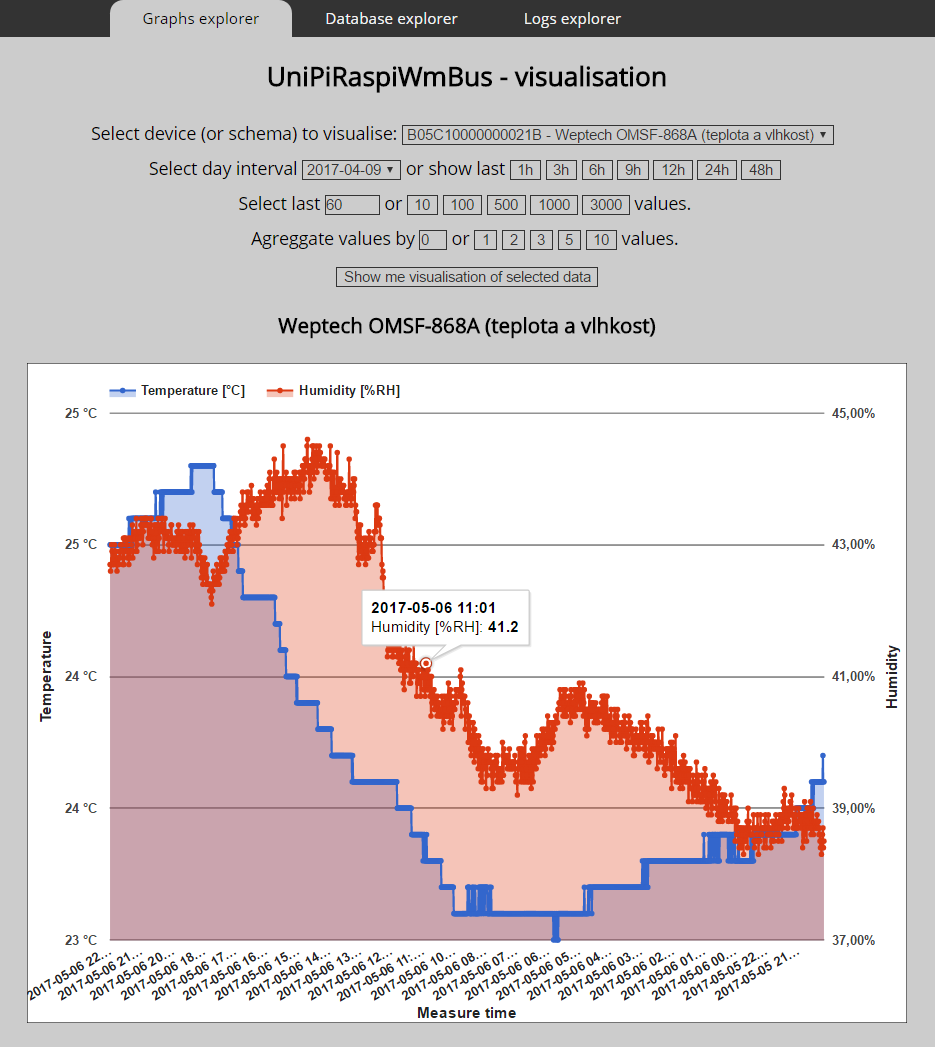
\includegraphics[scale=0.8]{obrazky/aplikace_vizualizace}
  \end{center}
	\vspace{-10pt}
	\caption{Snímek obrazovky vizualizační aplikace}
	\label{SectionVisualizaceDat}
\end{figure}
	\vspace{-10pt}
Záhlaví stránky obsahuje rozcestník:
\begin{itemize}
	\item Graphs explorer - Samotná vizualizační aplikace, popsaná v Kap.~\ref{SectionVizualizaceDat} a~\ref{SectionVizualizaceDat2}.
	\item Database explorer - Webový prohlížeč obsahu databáze, popsaný v Kap.~\ref{SectionUlozeniDatabaze} a~\ref{SectionUlozeniDatabaze2}.
	\item Logs explorer - Prohlížeč průběžných i chybových logů, zmíněný v Kap.~\ref{SectionUlozeniLogu}.
\end{itemize}

Stránka je rozdělena do dvou částí. V první části stránky se nachází formulář, pomocí kterého lze filtrovat data k vizualizaci:
\begin{itemize}
	\item výběr daného senzoru, případně schématu (spojení více senzorů do jednoho grafu),
	\item výběr dne k zobrazení,
	\item možnost zobrazení jen určitého počtu posledních hodnot daného čidla,
	\item možnost zobrazení jen určitého časového úseku příjmu daného čidla,
	\item možnost agregace hodnot. Tato volba umožňuje aproximaxi dat po zprůměrování několika následujících hodnot. Je určená pro orientační vykreslení dlouhého časového úseku s velkým množstvím hodnot,
	\item možnost automatického obnovení stránky v určitém intervalu.
\end{itemize}
 
Pod formulářem se nachází již vykreslený interaktivní graf.

Ukázky vizualizací zachycených dat (pro přehlednost přegenerovaných programem Matlab) jednotlivých zařízení jsou uvedeny v Příloze~\ref{PrilohaGrafy}.

\section{Shrnutí realizace}
Schéma výsledné realizace a vazby mezi jednotlivými HW a SW celky je zobrazeno na Obr.~\ref{SchemaFinal}.
\begin{figure}[!ht]
	\vspace{-10pt}
  \begin{center}
    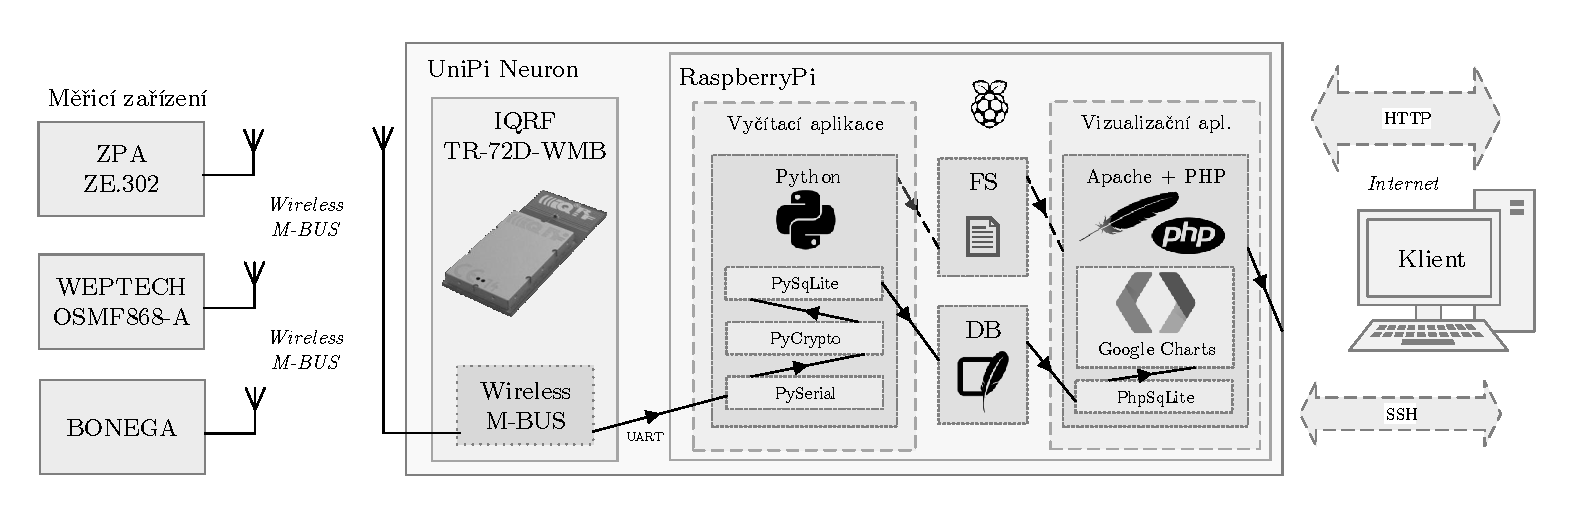
\includegraphics[scale=0.75]{obrazky/aplikace_schema}
  \end{center}
	\vspace{-50pt}
  \caption{Schéma výsledné realizace}
	\label{SchemaFinal}
	\vspace{-5pt}
\end{figure}



